\subsection{Balance General}

El balance general, junto con los estados de resultados, los cambios en el patrimonio y los flujos de efectivo, conforman los principales estados financieros. Su objetivo es brindar información relevante sobre la posición y el rendimiento financiero, así como sobre los movimientos de efectivo, para que diversos usuarios puedan tomar decisiones económicas fundamentadas.

La administración de la empresa es responsable de elaborar y presentar estos estados financieros.

En este apartado se presenta el Balance General, el cual muestra la situación financiera de la empresa al cierre de un periodo contable.

La estructura del balance general permite a los usuarios identificar aspectos como la liquidez, los plazos de los pasivos, la proporción de activos destinados a propiedades, planta y equipo, y la relación entre los recursos financiados por terceros y por los propietarios.

La liquidez de los activos se determina diferenciando entre activos corrientes y no corrientes. Los activos corrientes incluyen el efectivo y aquellos recursos que se espera convertir en efectivo mediante su venta o consumo en el plazo de un año o durante el ciclo operativo normal, si este es mayor. El ciclo operativo normal comprende desde la adquisición de inventarios, su procesamiento, la venta de los productos y el cobro correspondiente.

La situación financiera se expresa a través de los recursos disponibles, denominados activos, y las obligaciones sobre esos recursos, representadas por los pasivos y el patrimonio.

\begin{center}
    Patrimonio = Activos - Pasivos
\end{center}

En la tabla \ref{balanceGeneral} se presentan los activos, pasivos y patrimonio para cada año, comenzando en el año 0 con la inversión inicial que da inicio a las operaciones. Esta proyección incluye las ventas desde el primer año contable hasta el quinto.

El balance debe ser sometido a la aprobación de la Asamblea General de Accionistas por el Representante Legal, junto con los demás documentos requeridos por el artículo 446 del Código de Comercio. Dentro del plazo legal, el Representante Legal enviará a la Superintendencia, si corresponde, una copia del balance y sus anexos explicativos, junto con el acta de aprobación.

\vspace{2mm}
\begin{minipage}{0.8\textwidth}
\centering
\captionof{table}[{Balance General}]{ Balance General }
\label{balanceGeneral}
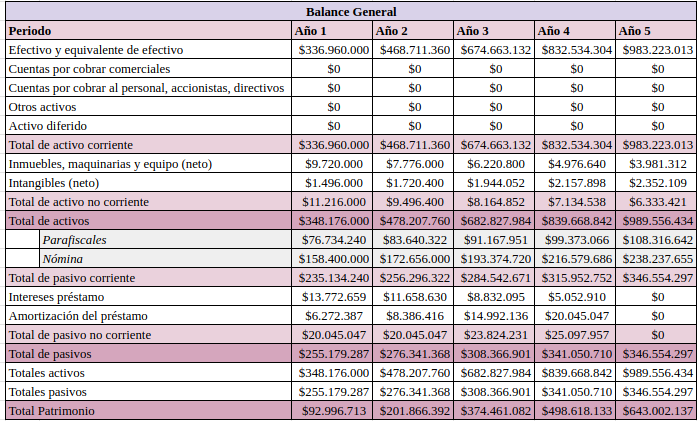
\includegraphics[width=0.9\textwidth]{Content/Images/AF/Balance_General.png}
\footnote{Nota. \textup{Fuente : Autores}}
\end{minipage}
\newpage